\subsubsection{Grundgleichungen einfacher Strukturelemente}

\begin{figure}[!htbp]
\centering
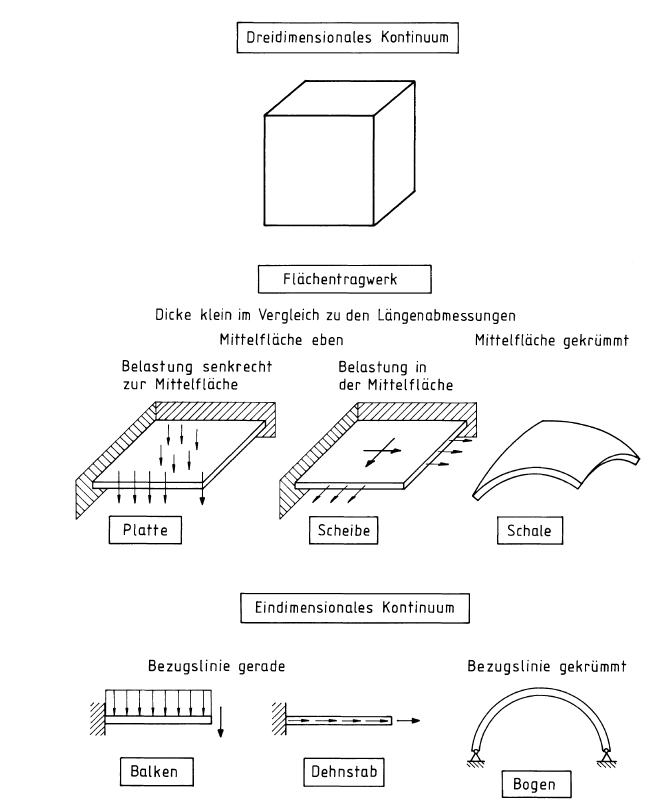
\includegraphics[width=0.75\linewidth]{files/Strukturelemente_Kno-8d4021870da8e52347739e58730bf650.png}
\caption[]{Übersicht über die Klassifizierung von Strukturvereinfachungen nach \cite{knothe1991finite}}
\label{strukturkontinua}
\end{figure}

Die im vorherigen Abschnitt eingeführten Feldgleichungen lassen sich für viele ingenieurwissenschaftliche Problemstellungen deutlich vereinfachen. In Figure~\ref{strukturkontinua} sind solche Vereinfachungen dargestellt.

Für die Impulsbilanz haben wir bereits in der Vorlesung zur ``Technischen Mechanik 2'' zwei Vereinfachungen kennengelernt:

\begin{itemize}
\item den Dehnstab
\item den Balken
\end{itemize}

Nachfolgend werden lediglich die Differentialgleichungen dieser beiden Strukturelemente eingeführt. Für eine Herleitung der Gleichungen sei auf die entsprechende Vorlesung verwiesen.

\paragraph{Differentialgleichung des Stabes}

Wird ein prismatisches Bauteil nur entlang seiner Achse $x$ belastet, so resultieren hieraus nur Normalspannungen $\sigma_x$. Solche Belastungsszenarien können über die Differentialgleichung des \textbf{Stabes} in guter Näherung beschrieben werden.

\begin{figure}[!htbp]
\centering
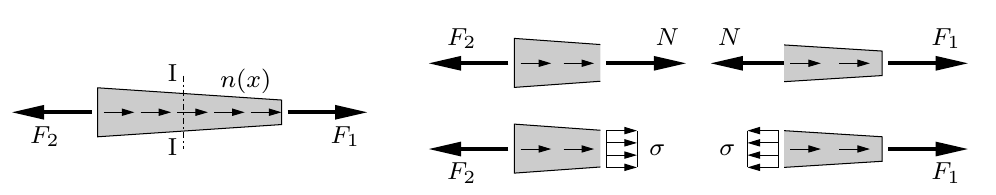
\includegraphics[width=0.75\linewidth]{files/Stab_TMKompakt-28bf6db8104e11c4fddde1fa0352bfd3.png}
\caption[]{Kräftegleichgewicht und Spannungen am geraden Stab nach \cite{wriggers2006technische}}
\label{stab}
\end{figure}

Die Differentialgleichung des Stabes lautet:

\begin{equation}
\label{stabdgl}
\frac{\text{d } \left( E(x)A(x) \frac{\text{d } u}{\text{d } x} \right) }{\text{d } x} =  \frac{\text{d } \left(E(x)A(x) \alpha_T(x) \Delta \theta\right)}{\text{d } x} - n(x)
\end{equation}
mit:

\begin{itemize}
\item $E$ - Elastizitätsmodul in MPa
\item $A$ - Querschnittsfläche in mm\textsuperscript{2}
\item $u$ - axiale Verschiebung in mm
\item $\alpha$ - Wärmeausdehnungskoeffizient in mm/K
\item $\Delta \theta$ - Temperaturänderung in K
\item $n$ - axiale Streckenlast in N/mm
\end{itemize}

Für einen konstanten $E$-Modul, eine konstante Querschnittsfläche $A$ sowie eine konstante Temperaturdifferenz $\Delta \theta$ kann diese Differentialgleichung vereinfacht werden zu:

\begin{equation}
\label{stabdglsimple}
 u^{\prime \prime} = \frac{\text{d}^2\,  u  }{\text{d } x^2} =  - \frac{n(x)}{EA}
\end{equation}

%  -+-+-+-+-+-+-AI-SPLIT

\paragraph{Differentialgleichung des Balkens}

Balken sind Tragstrukturen, die eindimensional modelliert werden, da ihre Breite und Höhe im Verhältnis zu ihrer Länge sehr gering sind. Im Unterschied zu Stäben, bei denen die Belastung nur in Längsrichtung erfolgt, werden Balken zusätzlich senkrecht zur Längsachse belastet. Dies führt dazu, dass in Stäben ausschlie$\beta$lich Normalkräfte auftreten, während sich in Balken Momente und Querkräfte als Schnittgrö$\beta$en ergeben.

\begin{figure}[!htbp]
\centering
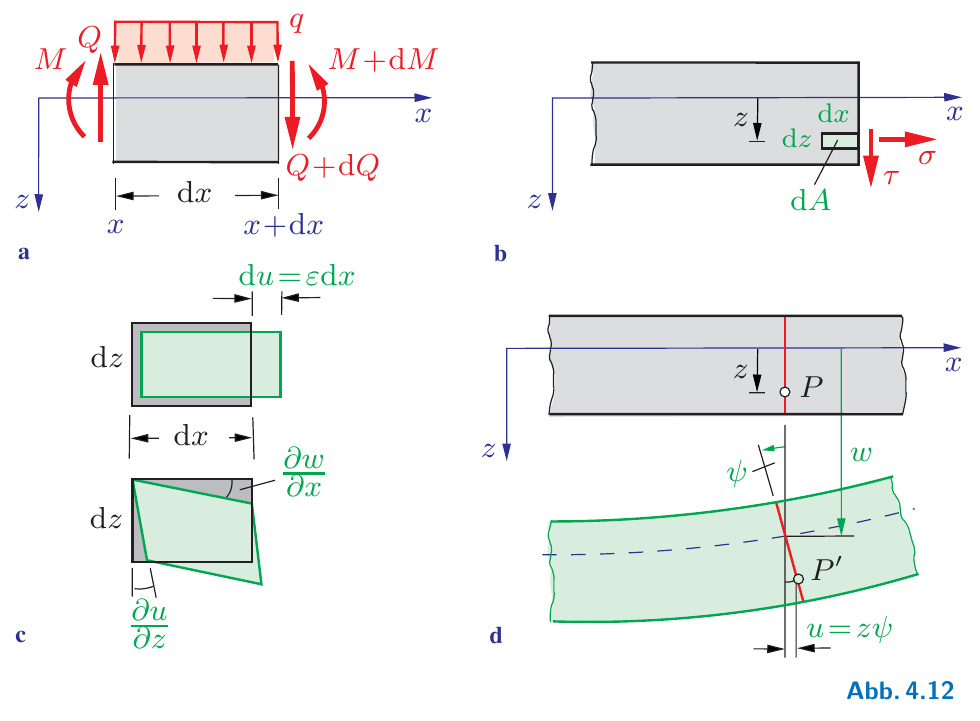
\includegraphics[width=0.75\linewidth]{files/Balken_TM2-bee88dc67566652ab2198dcf3f86b627.png}
\caption[]{Kräftegleichgewicht, Spannungen und Schnittgrö$\beta$en am geraden Balken nach \cite{gross2007technische}}
\label{balken}
\end{figure}

Die Differentialgleichung des Balkens lautet:

\begin{equation}
\label{balkendgl}
 \left(E I_y w^{\prime \prime}\right)^{\prime\prime} =  q(x)
\end{equation}
Für eine konstante Biegesteifigkeit $EI$ vereinfacht sich diese zu:
\begin{equation}
\label{balkendglsimple}
  w^{IV} =  \frac{q(x)}{E I_y}
\end{equation}